\documentclass[12pt]{article}
\usepackage[utf8]{inputenc}
\usepackage[OT2, T1, T2A]{fontenc}
\usepackage[russian]{babel}
\usepackage{graphicx}
\usepackage{geometry}
\usepackage{qrcode}
\usepackage{amsmath}
\usepackage{url}
\usepackage{minted}
\usepackage{pdfpages}
\geometry{margin=2cm}

% PLEASE NOTICE THAT, ACCORDING TO YOUR TITLE LENGTH, YOU MAY WANT TO ADAPT THE VSPACEs, SO THAT THE FINAL PAGE WILL BE PLEASING YOUR TASTE!%

\title{TitlePage}
\author{Your Name}
\date{Put the date}

\begin{document}

\begin{titlepage}
\begin{center}

    % Логотип
    
\includegraphics[width=0.25\textwidth]{Manas_logo.pdf} \\[1cm]
    
    % Университет и факультет
    \Large
    КЫРГЫЗ-ТҮРК ``МАНАС'' УНИВЕРСИТЕТИ \\[0.2cm]
    ТАБИГЫЙ ИЛИМДЕР ФАКУЛЬТЕТИ \\[0.2cm]
    КОЛДОНМО МАТЕМАТИКА ЖАНА ИНФОРМАТИКА \\[1cm]
    
    % Семестр и предмет
    \Large
    2025 -- 2026 КҮЗГҮ СЕМЕСТР \\[0.5cm]
    STJ -- 202 ОКУУ ПРАКТИКАСЫ САБАГЫ \\[1cm]
    
    % Тема отчёта
    \large
    \textbf{«ТЕЗ ЭСЕПТӨӨ ОЮНУ»} \\[0.3cm]
    ТЕМАСЫНДАГЫ ПРОЕКТТИН ОТЧЁТУ \\[1cm]
    
\end{center}

% Информация о студенте
\raggedright
\large
\begin{tabular}{ll}
Студенттин аты-жөнү: & Аскат Рахымбеков \\[0.5cm]
Курсу: & 3 \\[0.5cm]
Номери: & 2312.01002 \\[1cm]
Жетекчинин аты-жөнү: & Элла Абылаева \\[1.5cm]
\end{tabular}

\begin{center}
Бишкек 2025
\end{center}

\end{titlepage}

\section{Проекттин максаты жана жалпы мүнөздөмөсү}
\begin{itemize}
    \item Тез эсептөө оюнун иштеп чыгуу.
    \item Проект көңүл ачуу менен бирге \textbf{билим берүү} эффектин көздөйт: оюнчу оозеки эсепти, көңүл бурууну жана реакцияны оюндаштырылган форматта өнүктүрөт. Формат мектеп окуучуларына жана негизги арифметиканы кайталаган студенттерге ылайыктуу.
\end{itemize}

\section{Код}

\begin{itemize}
    \item Проекттин баштапкы коду \textbf{GitHub} репозиторийинде жеткиликтүү:  
\\\url{https://github.com/Hanbiike/math-snake}
    \item Иштетилген версиясы \textbf{GitHub Pages} аркылуу ачык:  
\\\url{https://hanbiike.github.io/math-snake/}
\end{itemize}


\begin{center}
\begin{tabular}{c@{\hspace{2cm}}c}
    \qrcode[height=3cm]{https://hanbiike.github.io/math-snake/} 
    & 
    \qrcode[height=3cm]{https://github.com/Hanbiike/math-snake} \\
    \small \textbf{Оюнду ачуу} & \small \textbf{GitHub репозиторийи} \\
\end{tabular}
\end{center}
\section{Интерфейс жана колдонуучу тажрыйбасы (UX)}
Барак үч негизги зонадан турат:
\begin{enumerate}
    \item \textbf{Жогорку панель (Header / HUD):} Режим (\textit{Mode}), татаалдык (\textit{Level}), упай (\textit{Score}), жандар (\textit{Lives}) жана (эгер күйгүзүлсө) таймер көрсөтүлөт.
    
    \item \textbf{Негизги талаа (Canvas):} 20×20 тордон турган оюн талаасында жылаан, жооп плиткалары жана декоративдик эффекттер чийилет. Үстүнө оверлейлер чыгышы мүмкүн: \textit{Main menu}, \textit{How to play}, \textit{Level Complete}, \textit{Game Over}.
    
    \item \textbf{Башкаруу элементтери:} Меню, Пауза жана мобайл үчүн экрандык \textit{D-pad}.
\end{enumerate}

\begin{center}
\begin{tabular}{@{}c@{\hspace{2cm}}c@{\hspace{2cm}}c@{}}
    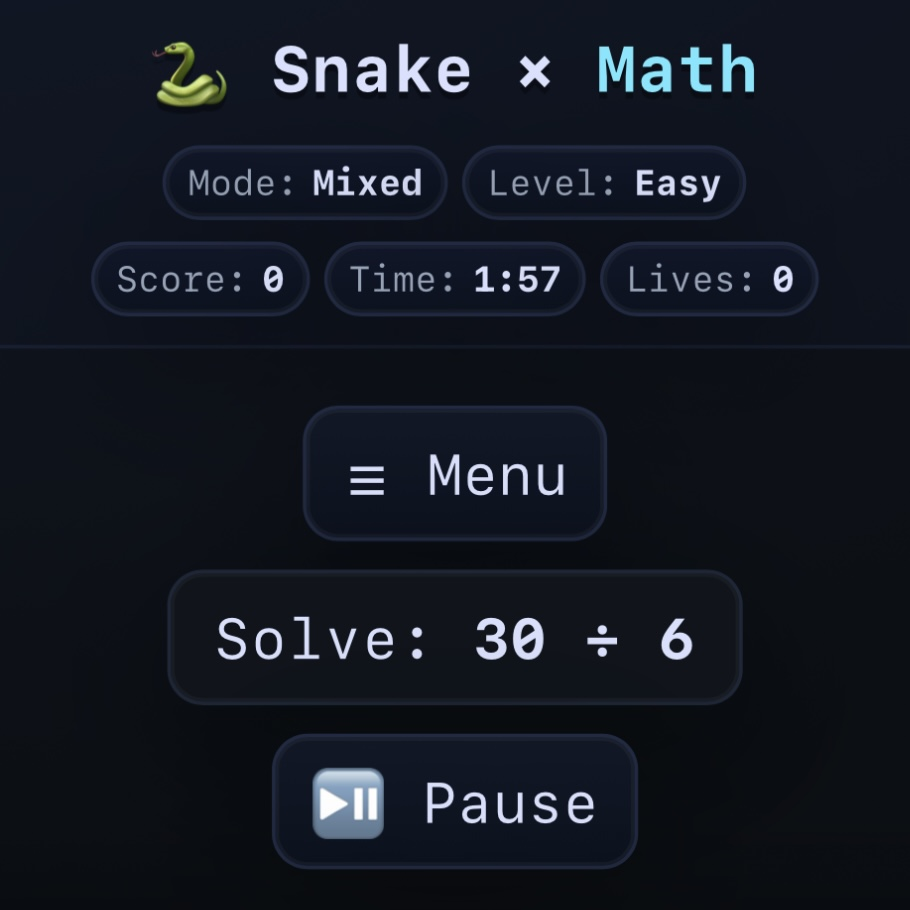
\includegraphics[width=0.25\textwidth]{IMG_3725.jpeg} &
    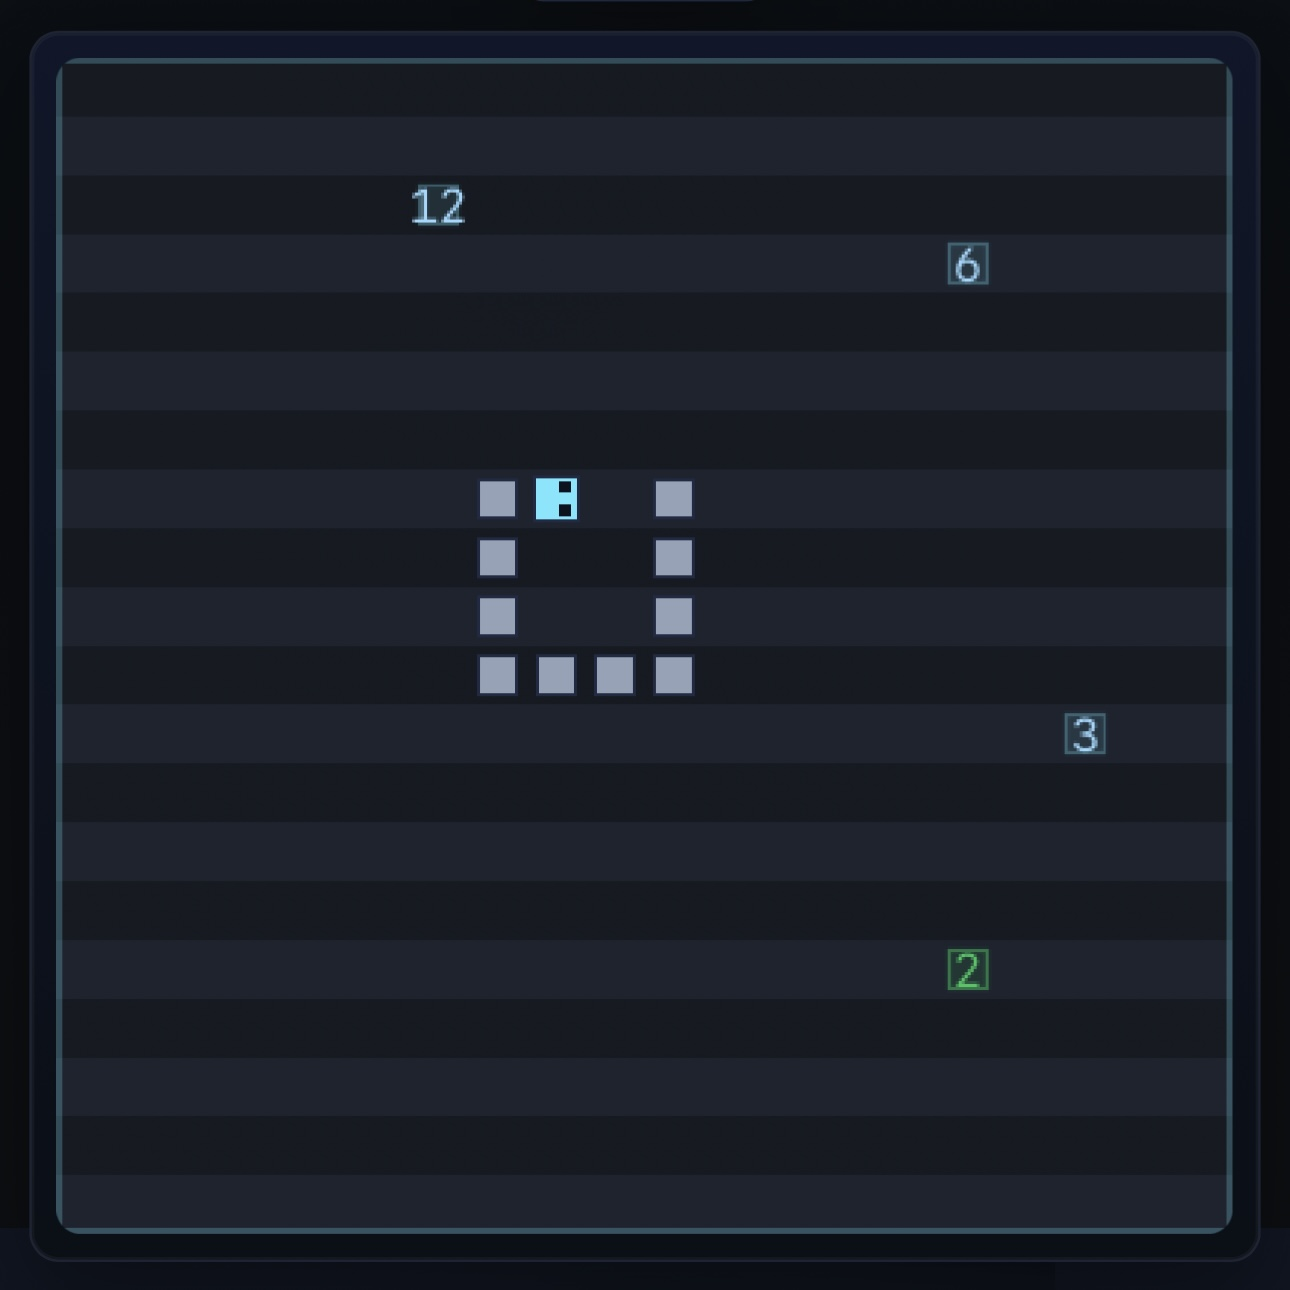
\includegraphics[width=0.25\textwidth]{IMG_3726.jpeg} &
    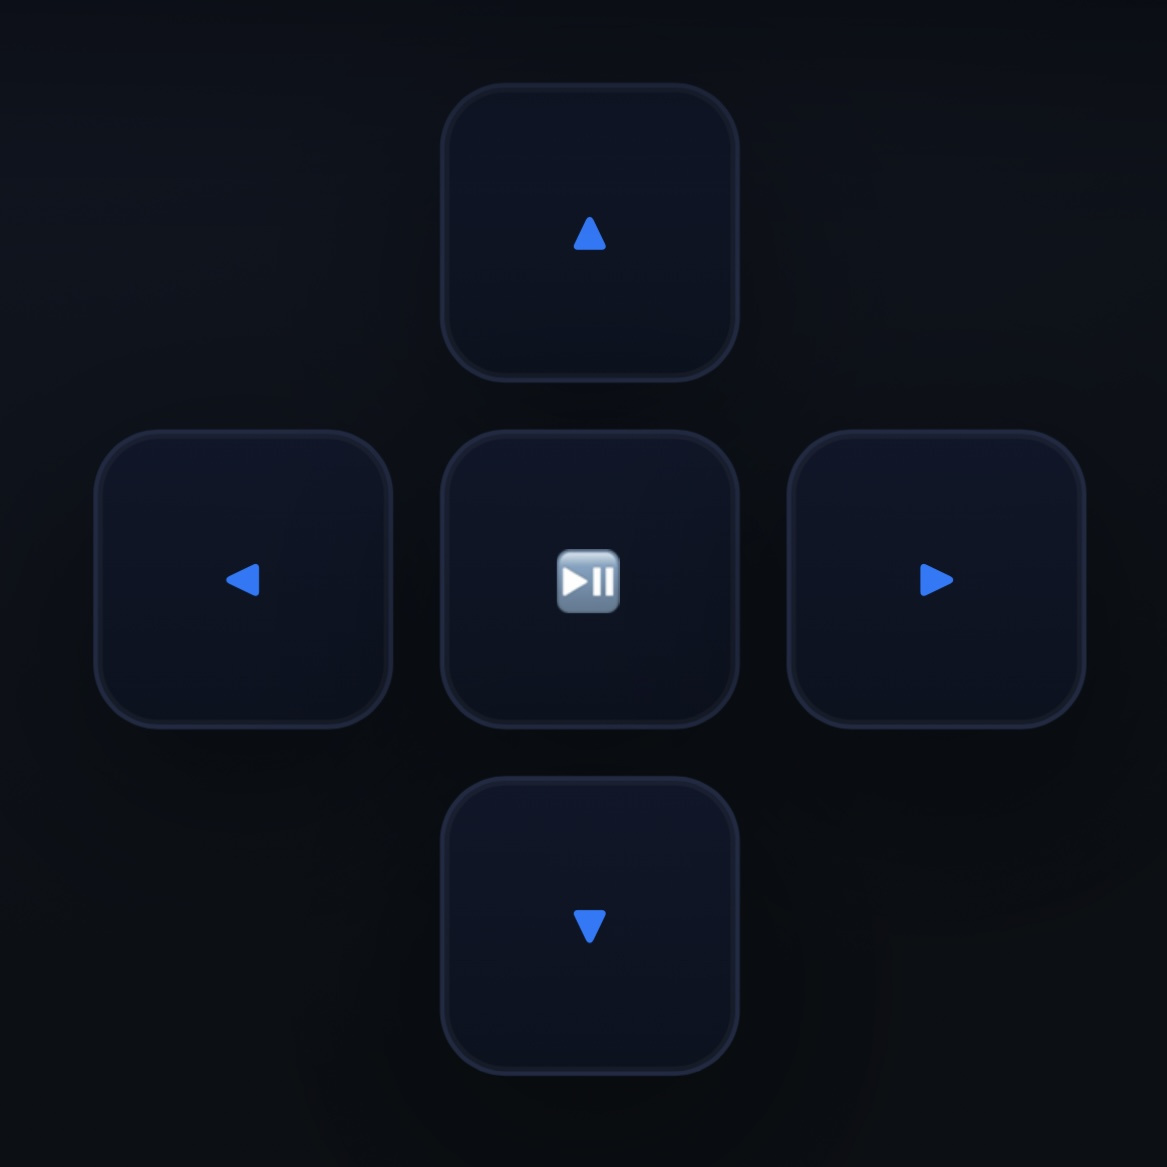
\includegraphics[width=0.25\textwidth]{IMG_3727.jpeg}
\end{tabular}
\end{center}

\section{Оюн логикасы}
Логиканын өзөгү \texttt{SnakeMathGame} классына топтолгон.

\subsection{Негизги параметрлер}
\begin{itemize}
  \item Тор өлчөмү: \textbf{20×20} клетка; клетка: \textbf{20 px}.
  \item Деңгээлди аяктоо үчүн туура жооптор: \textbf{10}.
  \item Баштапкы жандардын саны: \textbf{3}.
\end{itemize}

\subsection{Оюн режимдери}
\begin{itemize}
  \item \textbf{Addition} (кошуу), \textbf{Subtraction} (алып салуу), \textbf{Multiplication} (көбөйтүү), \textbf{Division} (калдыксыз бөлүү), \textbf{Mixed} (аралаш).
\end{itemize}

\subsection{Кыйынчылык деңгээлдери}
Деңгээл диапазондорго жана ылдамдыкка таасир этет:
\begin{itemize}
  \item \textbf{Easy} — бир орундуу; \textbf{Medium} — эки орундуу; \textbf{Mixed} — 1–99 аралаш; \textbf{Advanced} — үч орундууга чейин; \textbf{Expert} — тез оюн, ар бир туура жооптон кийин \textbf{ылдамдануу}.
\end{itemize}

\subsection{Мисалдарды түзүү жана жооп плиткалары}
\begin{itemize}
  \item Деңгээл башталганда туюнтма (\(a{+}b\), \(a{-}b\), \(a{\times}b\), \(a{\div}b\)) түзүлөт. Бөлүүдө жыйынтык дайыма \textbf{бүтүн} болушу үчүн \(a = b \cdot q\) принципи колдонулат.
  \item Талаада \textbf{4 позиция} тандалып, бирөөсүнө \textbf{туура жооп}, калгандарына \textbf{көңүлдү алаксытуучулар} коюлат.
  \item \textbf{Туура жооп} жегенде: упай +10, жылаандын узундугу +1; таймер күйүк болсо — \textbf{убакыт бонусу}; \textbf{Expert} деңгээлинде тик-интервал кыскарат (оюн тездейт).
  \item \textbf{Туура эмес} жооп — \textbf{жандардын саны -1}.
  \item \textbf{Sandbox mode} күйүк болсо, 10 туура жооп чектөөсү жок; болбосо 10го жеткенде \textit{деңгээл ийгиликтүү бүтүрүлдү}.
\end{itemize}

\subsection{Аяктоо шарттары}
\begin{itemize}
  \item Жандардын саны 0 болгондо — \textit{Game Over}.
  \item 10 туура жоопка жеткенде (Sandbox эмес) — \textit{Level Complete}.
\end{itemize}

\section{Башкаруу ыкмалары}
\begin{itemize}
  \item \textbf{Клавиатура:} жебелер же \textbf{WASD}; тескери бурулуп куйрукка урунбоо үчүн текшерүү бар.
  \item \textbf{Экрандык D-pad:} мобайл үчүн чоң баскычтар.
  \item \textbf{Сенсордук свайп}.
\end{itemize}

\section{Жыйынтык}
Бул проектте биз \textbf{«Math × Snake»} аттуу браузердик оюнду ишке ашырдык. Ал \textbf{JavaScript} (логика), \textbf{HTML5 Canvas} (графика) жана \textbf{CSS} (интерфейс) технологияларынын негизинде жазылды.  
Оюндун башкы идеясы — классикалык жылаан оюнунун механикасын арифметикалык машыгуу менен айкалыштыруу. Талаада кадимки «жемдин» ордуна бир нече \textbf{жооп варианттары} пайда болот, ал эми үстүңкү панелде \textbf{математикалык туюнтма} көрсөтүлөт. Оюнчу змейканы туура \textbf{жоопту жегенге} багытташы керек; туура эмес санды жесе — \textbf{жандары} кемийт.

Бул проект классикалык оюндук механиканы \textbf{эсеп чыгаруунун машыгуусу} менен айкалыштырып, окутууну оюндаштыруунун үлгүсүн көрсөтөт. Анын артыкчылыктары төмөнкүлөрдө көрүнөт:
\begin{itemize}
  \item \textbf{Арифметика:} оозеки эсептөөнү тездетип, математикалык көндүмдөрдү бекемдейт;
  \item \textbf{Көңүл топтоо жана реакция:} оюнчу туюнтманы чечип жатканда ошол эле учурда навигация кылат, бул параллелдүү ой жүгүртүүнү өнүктүрөт;
  \item \textbf{Оюндаштыруу:} окуу процессине кызыгууну арттырып, үзгүлтүксүз машыгууга түрткү берет.
\end{itemize}

Проекттин колдонуу чөйрөлөрү кеңири: мектеп сабактарында, машыгуу сабатында, онлайн-курстарда жана кошумча интерактивдүү курал катары пайдаланууга ылайыктуу. Ошентип, \textbf{«Math × Snake»} билим берүүнүн инновациялык форматы катары окутуу менен оюнду айкалыштырып, математика сабагына кызыгууну күчөтө алат.

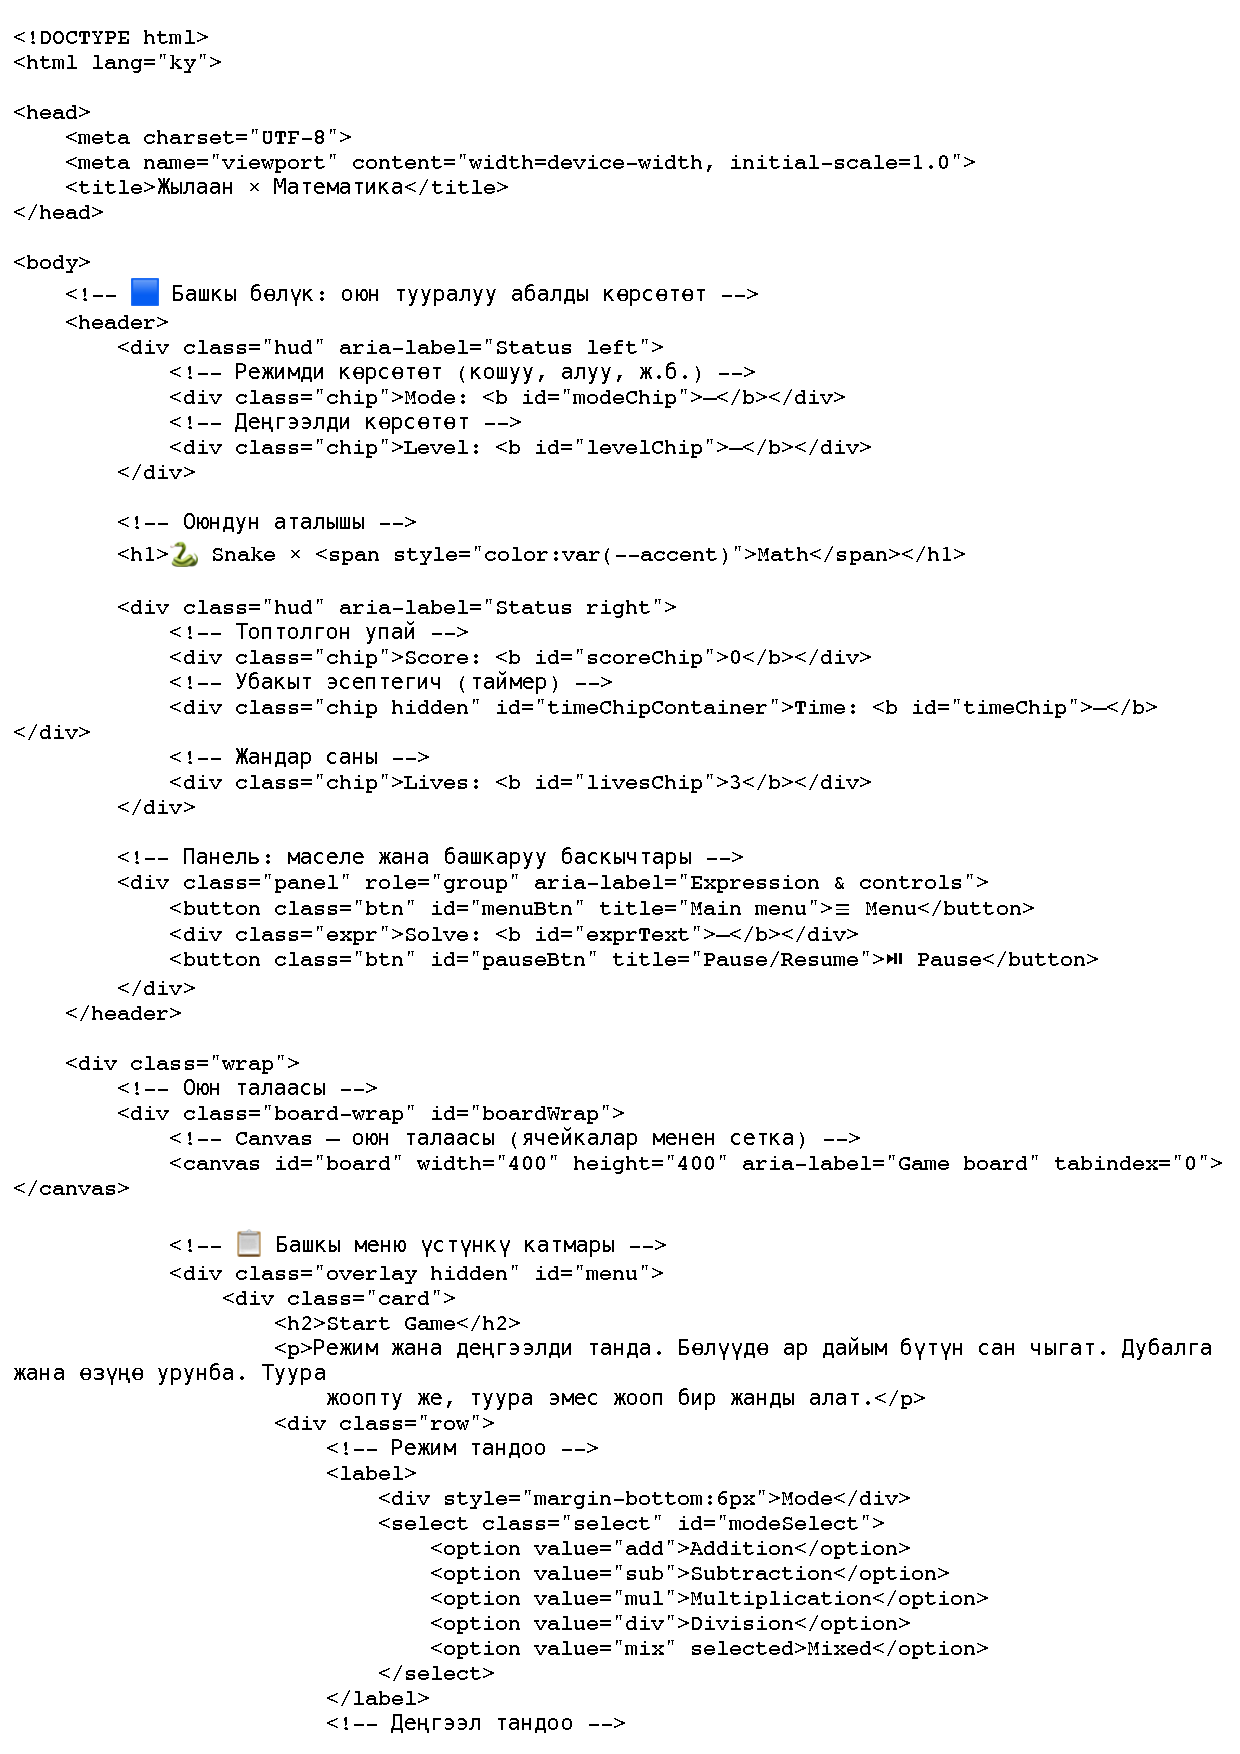
\includepdf[pages=1-10, frame, scale=0.95]{code.pdf}
\end{document}